\documentclass[a4paper]{article}


\usepackage[T1]{fontenc}    
\usepackage[utf8]{inputenc} 
\usepackage{textcomp}      
\date{} 					
\author{}                   
\usepackage{geometry}		
\geometry{ left=2cm, right=2cm, top=2cm, bottom=4cm, bindingoffset=5mm}

\usepackage{graphicx}
\usepackage{xcolor}
\usepackage{hyperref} 
\usepackage{fancyhdr}
\usepackage{amsmath}											
\pagestyle{fancy}
\fancyhf{}
\fancyhead[R]{2973140 - Felix Bühler  \\ 2893121 - Jan Leusmann \\  3141241 - Jamie Ullerich}
\fancyhead[L]{Scientific Visualisation \\ Sommersemester 2019 }
\renewcommand{\headrulewidth}{0.5pt} 				

\title{Exercise 7}

\begin{document}

\maketitle 
\thispagestyle{fancy}


\section*{Exercise 7.1 - Glyphs}


\section*{Exercis 7.2 - Isolines}

$f(-1.5, 1.5) = (-1.5 - 0.5)^{2} - 1.5^{2} =$ 1.75 = 1.8\\
$f(-0.5, 1.5) =$ -1.25 = -1.3\\
$f(0.5, 1.5) =$ -2.25 = -2.3\\
$f(1.5, 1.5) =$ -1.25 = -1.3\\
$f(-1.5, 0.5) =$ 3.75 = 3.8\\
$f(-0.5, 0.5) =$ 0.75 = 0.8\\
$f(0.5, 0.5) =$ -0.25 = -0.3\\
$f(1.5, 0.5) =$ 0.75 = 0.8\\
$f(-1.5, -0.5) =$ 3.75 = 3.8\\
$f(-0.5, -0.5) =$ 0.75 = 0.8\\
$f(0.5, -0.5) =$ -0.25 = -0.3\\
$f(1.5, -0.5) =$ 0.75 = 0.8 \\
$f(-1.5, -1.5) =$ 1.75 = 1.8 \\
$f(-0.5, -1.5) =$ -1.25 = -1.3\\
$f(0.5, -1.5) =$ -2.25 = -2.3\\
$f(1.5, -1.5) =$ -1.25 = -1.3\\

\begin{figure}[h!]
	\centering 
	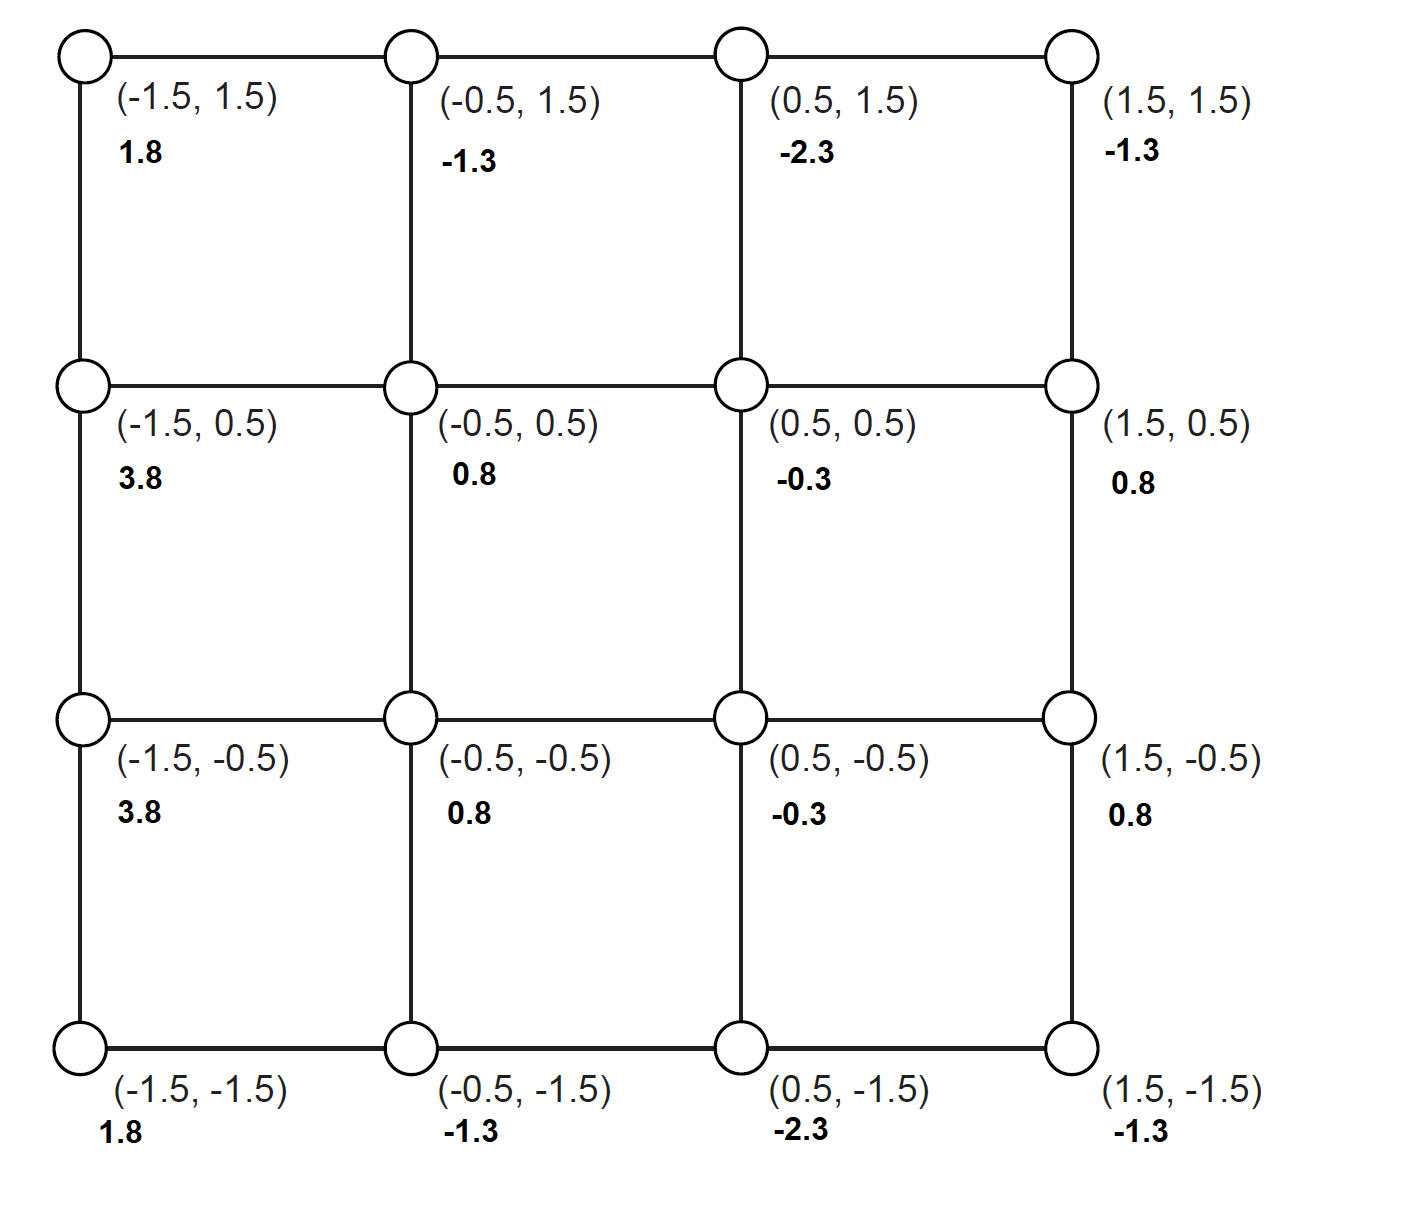
\includegraphics[width=11cm]{7_2_1.png}
	\caption{coordinates and function values }
	\label{fig:coordinates}
\end{figure}




\end{document}